In this section, we present \mad' performance model. Its goal is,
given a \mad assembly to be executed and the execution time of all the
transitions of all the components in the assembly, to estimate the total
execution time of the commissionning.
%
Intuitively, we automatically deduce the execution flow of a \mad
assembly based on \mad' formal semantics. This is done by generating a
dependency graph representing the execution flow of each \mad
component in the assembly and connecting them together according to their
dependencies (the connections between their ports). Then, a
\emph{source} vertex is connected to the vertices representing the beginning of
the execution of each component, and a \emph{sink} vertex is created to which
are connected the vertices representing the end of the execution of each
component.
%
Thus, a dependency graph representing the execution of the whole
assembly is obtained. By weighting the arcs corresponding to the transitions with
these transitions' individual execution time (and the other ones with 0),
we can find the total execution time of the assembly by finding the longest
path from the \emph{source} vertex to the \emph{sink} vertex.

\HC[HC]{why a performance model? give some motivations! 2 reasons,
  first a performance model offers a way to estimate the execution
  time of a commissioning which could be useful for sysadmins. second,
in this paper the performance model is used to validate the
experimental results and the quality of the prototype of \mad}

% By generating a graph modelling the execution flow of a \mad assembly,
% capturing both intra-component and inter-component dependencies, we
% reduce this problem to finding the longest path in a DAG.

%--------------------------------------
\subsection{Notations}
%--------------------------------------

Recall that given a component, we denote its set of places $\Pi$ and its
set of transitions $\Theta$. In the following, we consider that the
transitions go directly from a place to
another place instead of from an output dock to an input dock.
Hence, $\Theta$ is a multiset which elements are pairs of places.
%We
%can obtain the place corresponding to each dock by using the $place$
%function of the component.

In order to estimate the total commissionning time, we need to know
the execution time of each individual transition. In the following, we
consider the function $time\,:\,\Theta\rightarrow\mathbb{R}^{+}$
associating an execution time to each transition (taken as input). We
are aware that finding precise execution times of transitions is
difficult and the subject of many studies such as analytical
model~\cite{} or statistical studies~\cite{}. This point is left as
future work.

We also consider the following two functions:
\begin{itemize}
\item the \emph{group entrance function} $g_{in}\,:\,G\rightarrow\mathcal{P}\left(\Pi\right)$ with\\
$g_{in}(g)=\left\{ \pi\,\mid\,\pi\in g\land\exists\pi_{b}\,:\,\left(\pi_{b}\not\in g\land\left(\pi_{b},\pi\right)\in\Theta\right)\right\} $
(the result of $g_{in}$ is called the set of \emph{entrance places}
of the group)
\item the \emph{group exit function} $g_{out}\,:\,G\rightarrow\mathcal{P}\left(\Pi\right)$ with\\
$g_{out}(g)=\left\{ \pi\,\mid\,\pi\in g\land\exists\pi_{a}\,:\,\left(\pi_{a}\not\in g\land\left(\pi,\pi_{a}\right)\in\Theta\right)\right\} $
(the result of $g_{out}$ is called the set of \emph{exit places}
of the group)
\end{itemize}

Recall that an assembly is a tuple $\left(C,L_S,L_D\right)$. In
the following, for any component $c_i \in C$, any of its
associated set is denoted $X_i$, \eg $\Pi_i$ for the set of places of
the component $c_i$.
As previously for each set $X$ defining a component, we denote $X^*$ the
union (in the case of an assembly) or the extension (in the case of
a function) for all components. For instance:
\begin{itemize}
\item $\Pi^*=\bigcup_{i=1}^{n}\Pi_{i}$ (set of all \emph{places} in
the assembly)
\item $\left(time\right)^*\,:\,\Theta^*\rightarrow\mathbb{R}^{+}$
(function giving the \emph{execution time} of each transition) with:
$\left(time\right)^*\left(\theta\right)=\left(time\right)_{i}\left(\theta\right)$
if $\theta\in\Theta_{i}$ 
\end{itemize}
The execution flow graph is an oriented weighted graph \emph{$\left(V,A\right)$}
where $V$ is the set of vertices and $Ass$ is the multiset of weighted
arcs with elements in $V\times V\times\mathbb{R}^{+}$. We define
$V$ and $Ass$ in the following.

%--------------------------------------
\subsection{Vertices}
%--------------------------------------

For each place, we associate two vertices: one representing the place
itself and one representing the event of a token leaving the place.
\[
V_{\Pi}=\bigcup_{\pi\in\Pi^*}\left\{ v_\pi^\text{place},v_\pi^\text{leav}\right\} 
\]

For each transition, we associate two vertices: one representing the
beginning of the transition and one representing its end.
\[
V_{\Theta}=\bigcup_{\theta\in\Theta^*}\left\{ v_\theta^\text{beg},v_\theta^\text{end}\right\} 
\]

For each data-provide port we associate one vertex representing its activation.
\[
V_{D_p}=\bigcup_{p\in\left(D_p\right)^*}\left\{ v_p^\text{start}\right\} 
\]

For each service-provide port we associate two vertices: one representing
its activation and one its deactivation.
\[
V_{S_p}=\bigcup_{p\in\left(S_p\right)^*}\left\{ v_p^\text{start},v_p^\text{stop}\right\} 
\]

Finally, we define $V$ as the union of all these, plus one source
and one sink vertices. 
\[
V=V_{\Pi}\cup V_{\Theta}\cup V_{D_p}\cup V_{S_p}\cup\left\{ v^\text{source},v^\text{sink}\right\} 
\]

%--------------------------------------
\subsection{Arcs}
%--------------------------------------

In the dependency graph, arcs represent time constraints: the event represented
by the destination vertex must happen after the one represented by the source
vertex, at least $w$ seconds apart where $w$ is the weight of the arc. In
practice, the weight of all of the arcs except those corresponding to the
transitions is 0. The weights of the latter are the execution times of the
transitions.

For each place $\pi$ we associate one arc going from $v_\pi^\text{place}$ to
$v_\pi^\text{leav}$. This represents the fact that a token may leave $\pi$
only after it has entered it.
Figure~\ref{fig:place_graph} depicts the transformation of one place
\emph{running} to a dependency graph.
\[
A_{\Pi}=\bigcup_{\pi\in\Pi^*}\left\{ \left(v_\pi^\text{place},v_\pi^\text{leav},0\right)\right\} 
\]

%%%%%%%%%%%%%%%
\begin{figure}[h]
  \subfloat[\mad place]{%
    \fcolorbox{black!20}{white}{
      \begin{minipage}[c][2.5cm][c]{0.43\linewidth}%
        \centering
        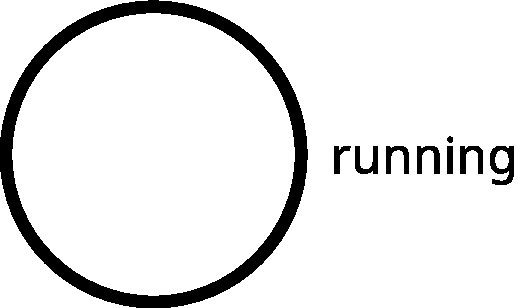
\includegraphics[scale=0.15]{images/perf_place.pdf}
      \end{minipage}
    }
  }
  \subfloat[Dependency graph]{%
    \fcolorbox{black!20}{white}{
      \begin{minipage}[c[c][2.5cm][c]{0.43\linewidth}%
        \centering
        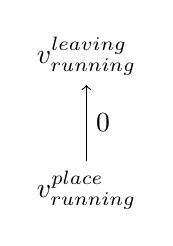
\begin{tikzpicture}[node distance=1.7cm]
          \node (leaving) [] {$v_\text{running}^\text{leaving}$};
          \node (place) [below of=leaving] {$v_\text{running}^\text{place}$};
          \draw [->] (place) -- (leaving) node[midway, right] {$0$};
        \end{tikzpicture}
      \end{minipage}
    }
  }
  \caption{A \mad place and its corresponding dependency graph}
  \label{fig:place_graph}
\end{figure}


For each transition $\theta$ going from $\pi_s$ to $\pi_d$, we associate
three arcs. The first between $v_\theta^\text{beg}$ and $v_\theta^\text{end}$
represents the fact that the end of $\theta$ happens at the time of the
start of $\theta$ plus its duration. The second between $v_{\pi_{s}}^\text{leav}$
and $v_\theta^\text{beg}$ represents the fact that $\theta$ may only
happen after a token leaved $\pi_s$. The third one between $v_\theta^\text{end}$ and
$v_{\pi_{d}}^\text{place}$ represents the fact that a token may enter $\pi_d$ only
after $\theta$ has finished.
Figure~\ref{fig:transition_graph} depicts the transformation of three
transitions \emph{t1}, \emph{t2} and \emph{t3} to a dependency graph.
\begin{align*}
A_{\Theta}=\bigcup_{\theta=\left(\pi_{s},\pi_{d}\right)\in\Theta^*} & \left\{ \left(v_\theta^\text{beg},v_\theta^\text{end},time^*\left(\theta\right)\right),\right.\\
 & \left(v_{\pi_{s}}^\text{leav},v_\theta^\text{beg},0\right),\left. \left(v_\theta^\text{end},v_{\pi_{d}}^\text{place},0\right)\right\}
\end{align*}

%%%%%%%%%%%%%%%
\begin{figure}[h]
  \subfloat[\mad internal net example]{
    \fcolorbox{black!20}{white}{
      \begin{minipage}[c][7.5cm][c]{0.33\linewidth}%
        \centering
        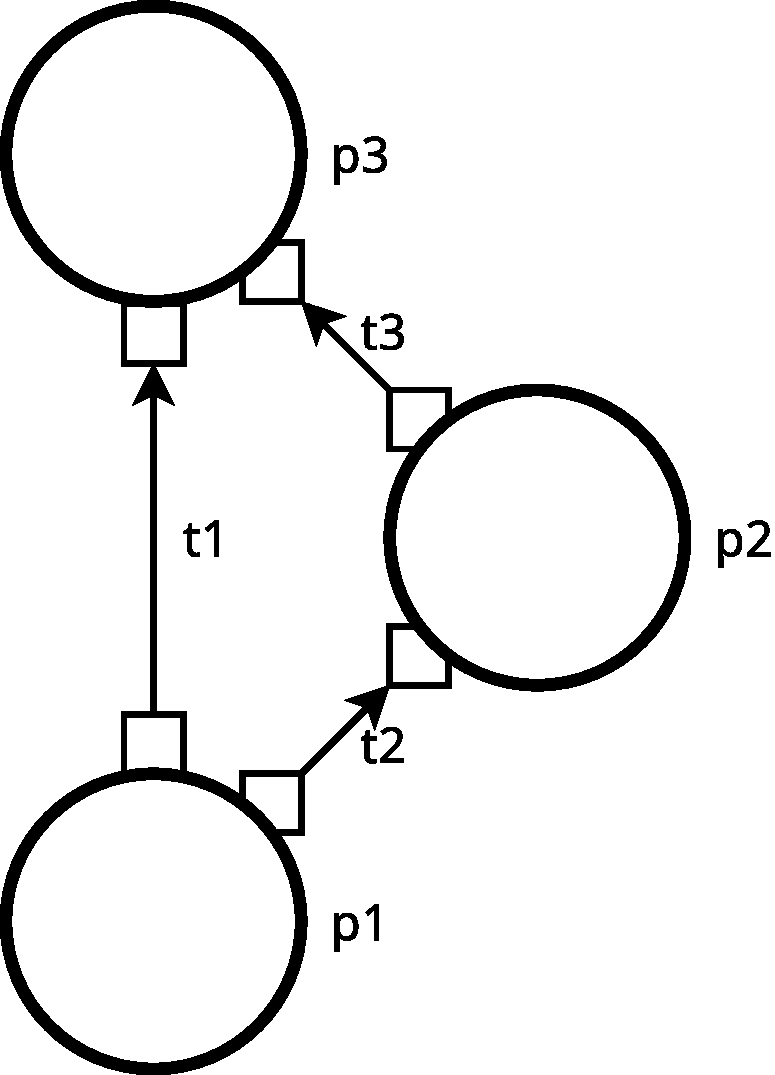
\includegraphics[width=0.8\columnwidth]{images/perf_transition.pdf} \label{fig:transmadeus}
      \end{minipage}
    }
  }
  \subfloat[Dependency graph]{
    \fcolorbox{black!20}{white}{
      \begin{minipage}[c][7.5cm][c]{0.53\linewidth}%
        \centering
        \begin{tikzpicture}[node distance=1.7cm]
          \node (p3l) [] {$v_\text{p3}^\text{leav}$};
          \node (p3) [below =15pt of p3l] {$v_\text{p3}^\text{place}$};
          \node (t1e) [below =15pt of p3] {$v_\text{t1}^\text{end}$};
          \node (t1) [below =15pt of t1e] {$v_\text{t1}^\text{beg}$};
          \node (p1l) [below =15pt of t1] {$v_\text{p1}^\text{leav}$};
          \node (p1) [below =15pt of p1l] {$v_\text{p1}^\text{place}$};
          \node (t2) [right =25pt of p1l] {$v_\text{t2}^\text{beg}$};
          \node (t2e) [right =25pt of t2] {$v_\text{t2}^\text{end}$};
          \node (p2) [above =15pt of t2e] {$v_\text{p2}^\text{place}$};
          \node (p2l) [above =15pt of p2] {$v_\text{p2}^\text{leav}$};
          \node (t3) [above =15pt of p2l] {$v_\text{t3}^\text{beg}$};
          \node (t3e) [right =15pt of p3] {$v_\text{t3}^\text{end}$};
          \draw [->] (p3) -- (p3l) node[midway, right, scale=0.7] {$0$};
          \draw [->] (p2) -- (p2l) node[midway, right, scale=0.7] {$0$};
          \draw [->] (p1) -- (p1l) node[midway, right, scale=0.7] {$0$};
          \draw [->] (t3) -- (t3e) node[midway, above, scale=0.7] {$time(\text{t3})$};
          \draw [->] (t2) -- (t2e) node[midway, below, scale=0.7] {$time(\text{t2})$};
          \draw [->] (t1) -- (t1e) node[midway, right, scale=0.7] {$time(\text{t1})$};
          \draw [->] (p1l) -- (t1) node[midway, right, scale=0.7] {$0$};
          \draw [->] (p1l) -- (t2) node[midway, below, scale=0.7] {$0$};
          \draw [->] (p2l) -- (t3) node[midway, right, scale=0.7] {$0$};
          \draw [->] (t1e) -- (p3) node[midway, right, scale=0.7] {$0$};
          \draw [->] (t2e) -- (p2) node[midway, right, scale=0.7] {$0$};
          \draw [->] (t3e) -- (p3) node[midway, above, scale=0.7] {$0$};
        \end{tikzpicture}
        \label{fig:transdag}
      \end{minipage}
    }
  }
  \caption{Example of a set of \mad transitions translated to its equivalent dependency graph}
  \label{fig:transition_graph}
\end{figure}


For each data-provide port $p$, we associate (a) for each binding between
$p$ and a place $\pi$ one arc going from $v_\pi^\text{place}$ to
$v_p^\text{start}$, and (b) for each connection connecting $p$
to a data-use port $u$, for each binding between $u$ and a transition
$\theta$ one arc going from $v_p^\text{start}$ to $v_\theta^\text{beg}$.
The (a) arcs represent the fact that the data becomes
available when a place bound to it is reached. The (b) arcs represent the
fact that the transitions bound to a data-use port may only execute once
the port is provided.
Figure~\ref{fig:data_ports_graph} depicts the transformation of a
data-provide port \emph{dp} bound to place \emph{c1p} and connected to
data-use port \emph{du} which is bound to transition \emph{c2t}.
\begin{align*}
A_{D}=\bigcup_{p\in D_p}
& \left(\bigcup_{\pi,\,\left(p,\pi\right)\in B_{D_{p}}^*}\left\{ \left(v_\pi^\text{place},v_p^\text{start},0\right)\right\}\right. \\
& \left.\cup\bigcup_{\substack{u,\,\left(u,p\right)\in L_D \\
  \theta,\,\left(u,\theta\right)\in B_{D_{u}}^*}}\left\{ \left(v_p^\text{start},v_\theta^\text{beg},0\right)\right\}\right)
\end{align*}

%%%%%%%%%%%%%%%
\begin{figure}[h]
  \subfloat[Madeus data connection]{%
    \fcolorbox{black!20}{white}{
      \begin{minipage}[c][5cm][c]{0.34\linewidth}%
        \centering
        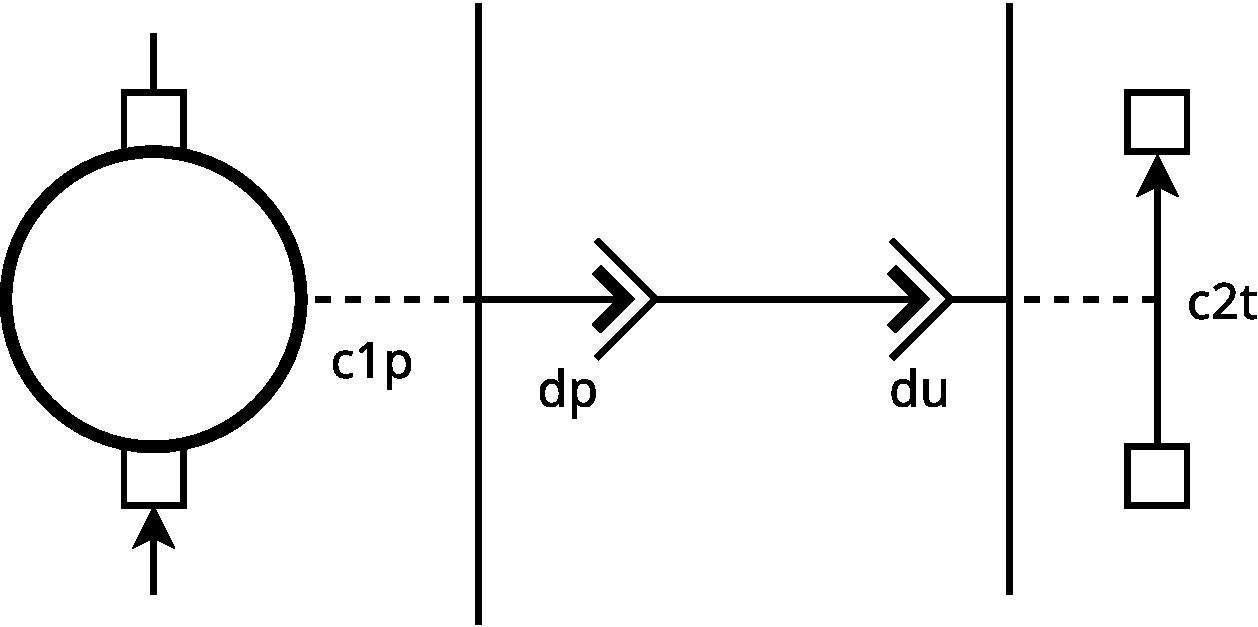
\includegraphics[scale=0.14]{images/perf_data_ports.pdf}
        \label{fig:dataport}
      \end{minipage}
    }
  }
  \subfloat[Dependency graph]{%
    \fcolorbox{black!20}{white}{
      \begin{minipage}[c][5cm][c]{0.52\linewidth}%
        \centering
        \begin{tikzpicture}[node distance=1.7cm]
          \node (c1t2) [] {$v_\text{c1t2}^\text{beg}$};
          \node (c1p1l) [below =15pt of c1t2] {$v_\text{c1p}^\text{leav}$};
          \node (c1p1) [below =15pt of c1p1l] {$v_\text{c1p}^\text{place}$};
          \node (c1t1_end) [below=15pt of c1p1] {$v_\text{c1t1}^\text{end}$};
          \draw [->] (c1t1_end) -- (c1p1) node[midway, right, scale=0.7] {$0$};
          \draw [->] (c1p1) -- (c1p1l) node[midway, right, scale=0.7] {$0$};
          \draw [->] (c1p1l) -- (c1t2) node[midway, right, scale=0.7] {$0$};
          \node (dp) [right =15pt of c1p1] {$v_\text{dp}^\text{start}$};
          \node (c2t) [right =15pt of dp] {$v_\text{c2t}^\text{beg}$};
          \node (c2t_end) [above =15pt of c2t] {$v_\text{c2t}^\text{end}$};
          \draw [->] (c2t) -- (c2t_end) node[midway, right, scale=0.7] {$time(\text{c2t})$};
          \draw [->] (c1p1) -- (dp) node[midway, below, scale=0.7] {$0$};
          \draw [->] (dp) -- (c2t) node[midway, below, scale=0.7] {$0$};
        \end{tikzpicture}
        \label{fig:dataportdag}
      \end{minipage}
    }
  }
  \caption{A data-use-provide connection and its corresponding
    dependency graph}
  \label{fig:data_ports_graph}
\end{figure}


For each service-provide port $p$, we associate (a) for each binding between
$p$ and a group $g$ one arc going from $v_\pi^\text{place}$ to $v_p^\text{start}$
for each $\pi$ in $g_{in}(g)$ and one arc going from $v_p^\text{stop}$ to
$v_\pi^\text{leav}$ for each place $\pi$ $g_{out}(g)$, and (b) for each
connection connecting $p$ to a service-use port $u$, for each binding between
$u$ and a transition $\theta$ one arc going from $v_p^\text{start}$ to
$v_\theta^\text{beg}$ and one arc going from $v_\theta^\text{end}$ to
$v_p^\text{stop}$.
The (a) arcs represent the fact that the service becomes available when all
groups bound to it have a token, and each of them can be deactivated only when
the provide port is not used anymore. The (b) arcs represent the
fact that the transitions bound to a service-use port may only execute once
the port is provided, and do not use the port anymore once they are over.
Figure~\ref{fig:service_ports_graph} depicts the transformation of a
service-provide port \emph{sp} bound to a group with \emph{c1p1} as entrance
place and \emph{c1p2} as exit place, and connected to service-use port
\emph{su} which is bound to transition \emph{c2t}.

\begin{alignat*}{3}
A_{S}=\bigcup_{p\in S_p}
& \left(\bigcup_{g,\,\left(p,g\right)\in B_{S_{p}}^*} \right. && \left. \left(\bigcup_{\pi\in g_{in}(g)} \left\{\left(v_\pi^\text{place},v_p^\text{start},0\right)\right\}\right.\right. \\
&&& \left. \cup\left.\bigcup_{\pi\in g_{out}(g)} \left\{\left(v_p^\text{stop},v_\pi^\text{leav},0\right)\right\}\right)\right. \\
& \left.\cup\bigcup_{\substack{u,\,\left(u,p\right)\in L_S \\
      \theta,\,\left(u,\theta\right)\in B_{S_{u}}^*}} \right. && \left. \left\{ \left(v_p^\text{start},v_\theta^\text{beg},0\right),\right.\right. \left.\left.\left(v_\theta^\text{end},v_p^\text{stop},0\right)\right.\Big\}\right.\Bigg)
\end{alignat*}

%%%%%%%%%%%%%%%
\begin{figure}[t]
  \subfloat[\mad use-provide connection]{%
    \fcolorbox{black!20}{white}{
      \begin{minipage}[c]{0.95\columnwidth}%
        \centering
        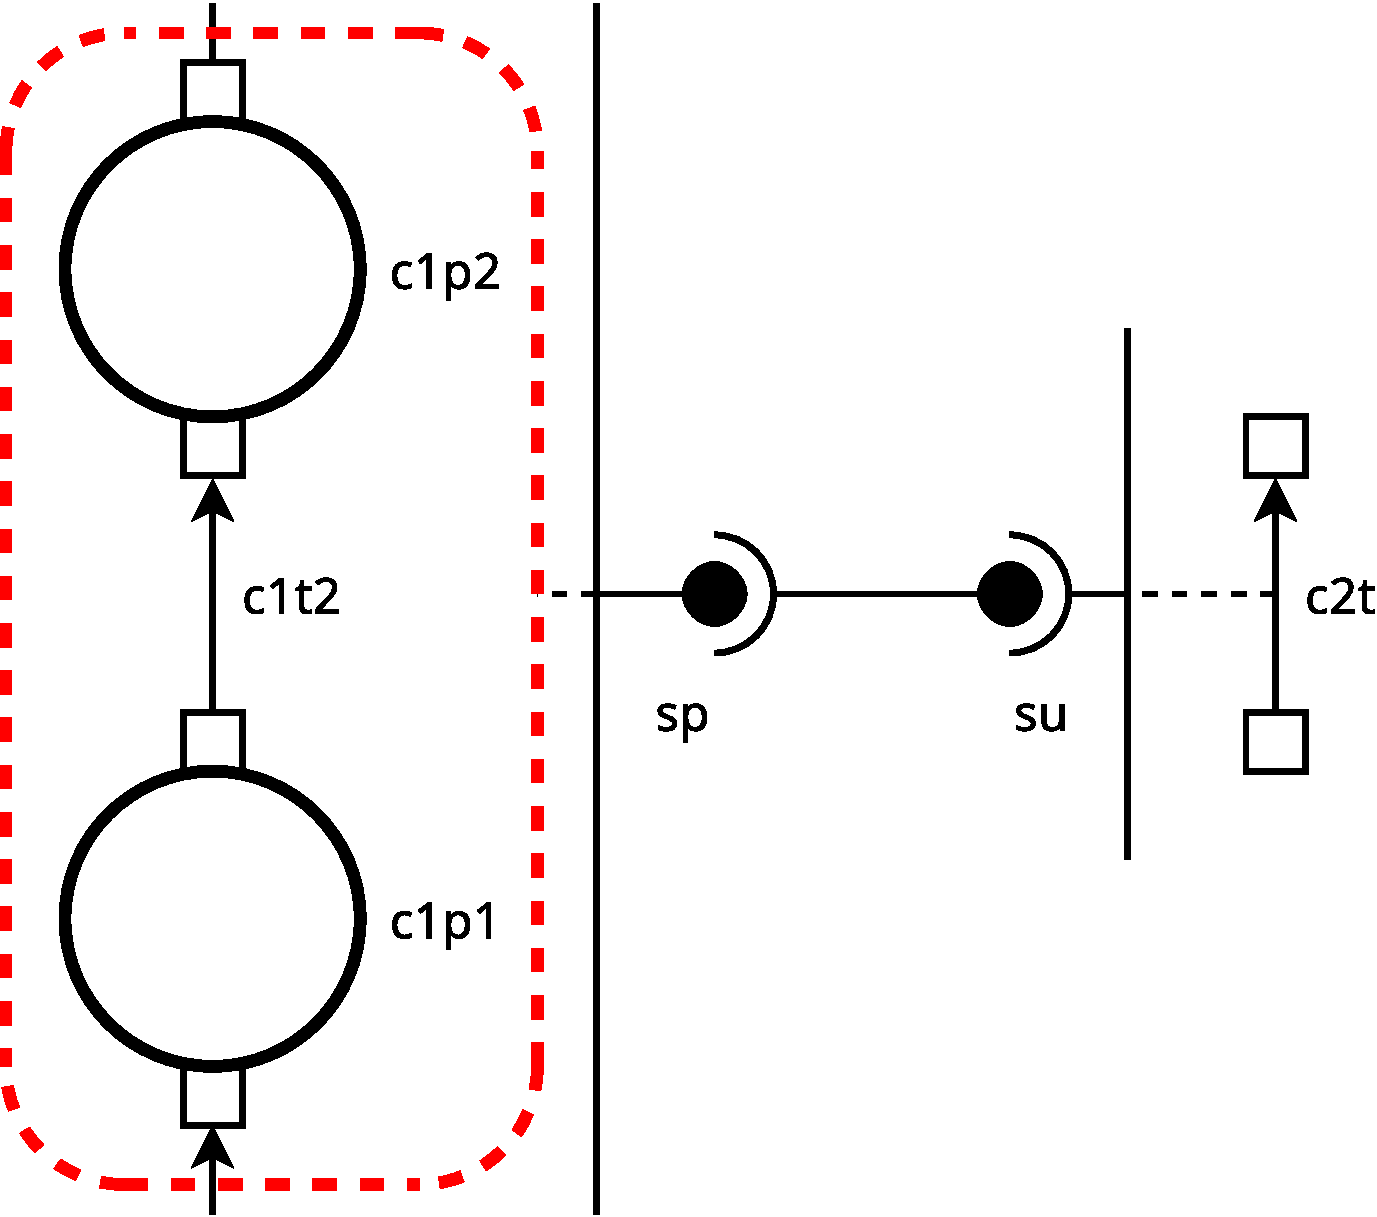
\includegraphics[scale=0.15]{images/perf_service_ports.pdf}
      \end{minipage}
    }
  }
  \\

  \subfloat[Dependency graph]{%
    \fcolorbox{black!20}{white}{
      \begin{minipage}[c]{0.95\columnwidth}%
        \centering
        \begin{tikzpicture}[node distance=1.7cm]
          \node (c1t3) [] {$v_\text{c1t3}^\text{beg}$};
          \node (c1p2l) [below =15pt of c1t3] {$v_\text{c1p2}^\text{leav}$};
          \node (c1p2) [below =15pt of c1p2l] {$v_\text{c1p2}^\text{place}$};
          \node (c1t2_end) [below =15pt of c1p2] {$v_\text{c1t2}^\text{end}$};
          \node (c1t2) [below =15pt of c1t2_end] {$v_\text{c1t2}^\text{beg}$};
          \node (c1p1l) [below =15pt of c1t2] {$v_\text{c1p1}^\text{leav}$};
          \node (c1p1) [below =15pt of c1p1l] {$v_\text{c1p1}^\text{place}$};
          \node (c1t1_end) [below =15pt of c1p1] {$v_\text{c1t1}^\text{end}$};
          \draw [->] (c1t1_end) -- (c1p1) node[midway, right, scale=0.7] {$0$};
          \draw [->] (c1p1) -- (c1p1l) node[midway, right, scale=0.7] {$0$};
          \draw [->] (c1p1l) -- (c1t2) node[midway, right, scale=0.7] {$0$};
          \draw [->] (c1t2) -- (c1t2_end) node[midway, right, scale=0.7] {$time(\text{c1t2})$};
          \draw [->] (c1t2_end) -- (c1p2) node[midway, right, scale=0.7] {$0$};
          \draw [->] (c1p2) -- (c1p2l) node[midway, right, scale=0.7] {$0$};
          \draw [->] (c1p2l) -- (c1t3) node[midway, right, scale=0.7] {$0$};
          \node (sp) [right =20pt of c1p1] {$v_\text{sp}^\text{start}$};
          \node (c2t) [right =20pt of sp] {$v_\text{c2t}^\text{beginning}$};
          \node (c2t_end) [above =15pt of c2t] {$v_\text{c2t}^\text{end}$};
          \node (sps) [right =20pt of c1p2l] {$v_\text{sp}^\text{stop}$};
          \draw [->] (c2t) -- (c2t_end) node[midway, right, scale=0.7] {$time(\text{c2t})$};
          \draw [->] (c1p1) -- (sp) node[midway, below, scale=0.7] {$0$};
          \draw [->] (sp) -- (c2t) node[midway, below, scale=0.7] {$0$};
          \draw [->] (c2t_end) to[bend right] node[midway, right, scale=0.7] {$0$}(sps.east) ;
          \draw [->] (sps) -- (c1p2l) node[midway, above, scale=0.7] {$0$};
        \end{tikzpicture}
      \end{minipage}
    }
  }
  \caption{Vertices and arcs for service ports, bindings and connections}
  \label{fig:service_ports_graph}
\end{figure}

For each initial place $\pi$ we associate one arc going from $v^\text{source}$
 to $v_\pi^\text{place}$, representing the fact that a token is placed in each
 initial place at the very beginning.
Figure~\ref{fig:source_sink_graph} depicts the transformation of two initial
places \emph{c1p1} and \emph{c2p2}.
\[
A_{I}=\bigcup_{\pi\in I^*}\left\{ \left(v^\text{source},v_\pi^\text{place},0\right)\right\} 
\]

In addition to the set of all initial places $I^*$, we define
the set of all final places $F^*$ as the set of places which
do not have any outgoing transition. Formally,
$F^*=\left\{ \pi\,\mid\,\pi\in\Pi^*\land\lnot\left(\exists\pi_{a}\in\Pi^*\,:\,\left(\pi,\pi_{a}\right)\in\Theta^*\right)\right\} $.
Then, for each final place $\pi$ we associate one arc going from
$v_\pi^\text{place}$ to $v^\text{sink}$, representing the fact that the
commissionning is over only after all components have reached their final places
(\ie when no more transition can be executed).
Figure~\ref{fig:source_sink_graph} depicts the transformation of three final
places \emph{c1p2}, \emph{c2p2} and \emph{c2p3}.
\[
A_F=\bigcup_{\pi\in F^*}\left\{ v_\pi^\text{place},v^\text{sink},0\right\} 
\]

%%%%%%%%%%%%%%%
\begin{figure}[t]
  \subfloat[\mad assembly]{%
    \begin{minipage}[c]{0.95\columnwidth}%
      \centering
      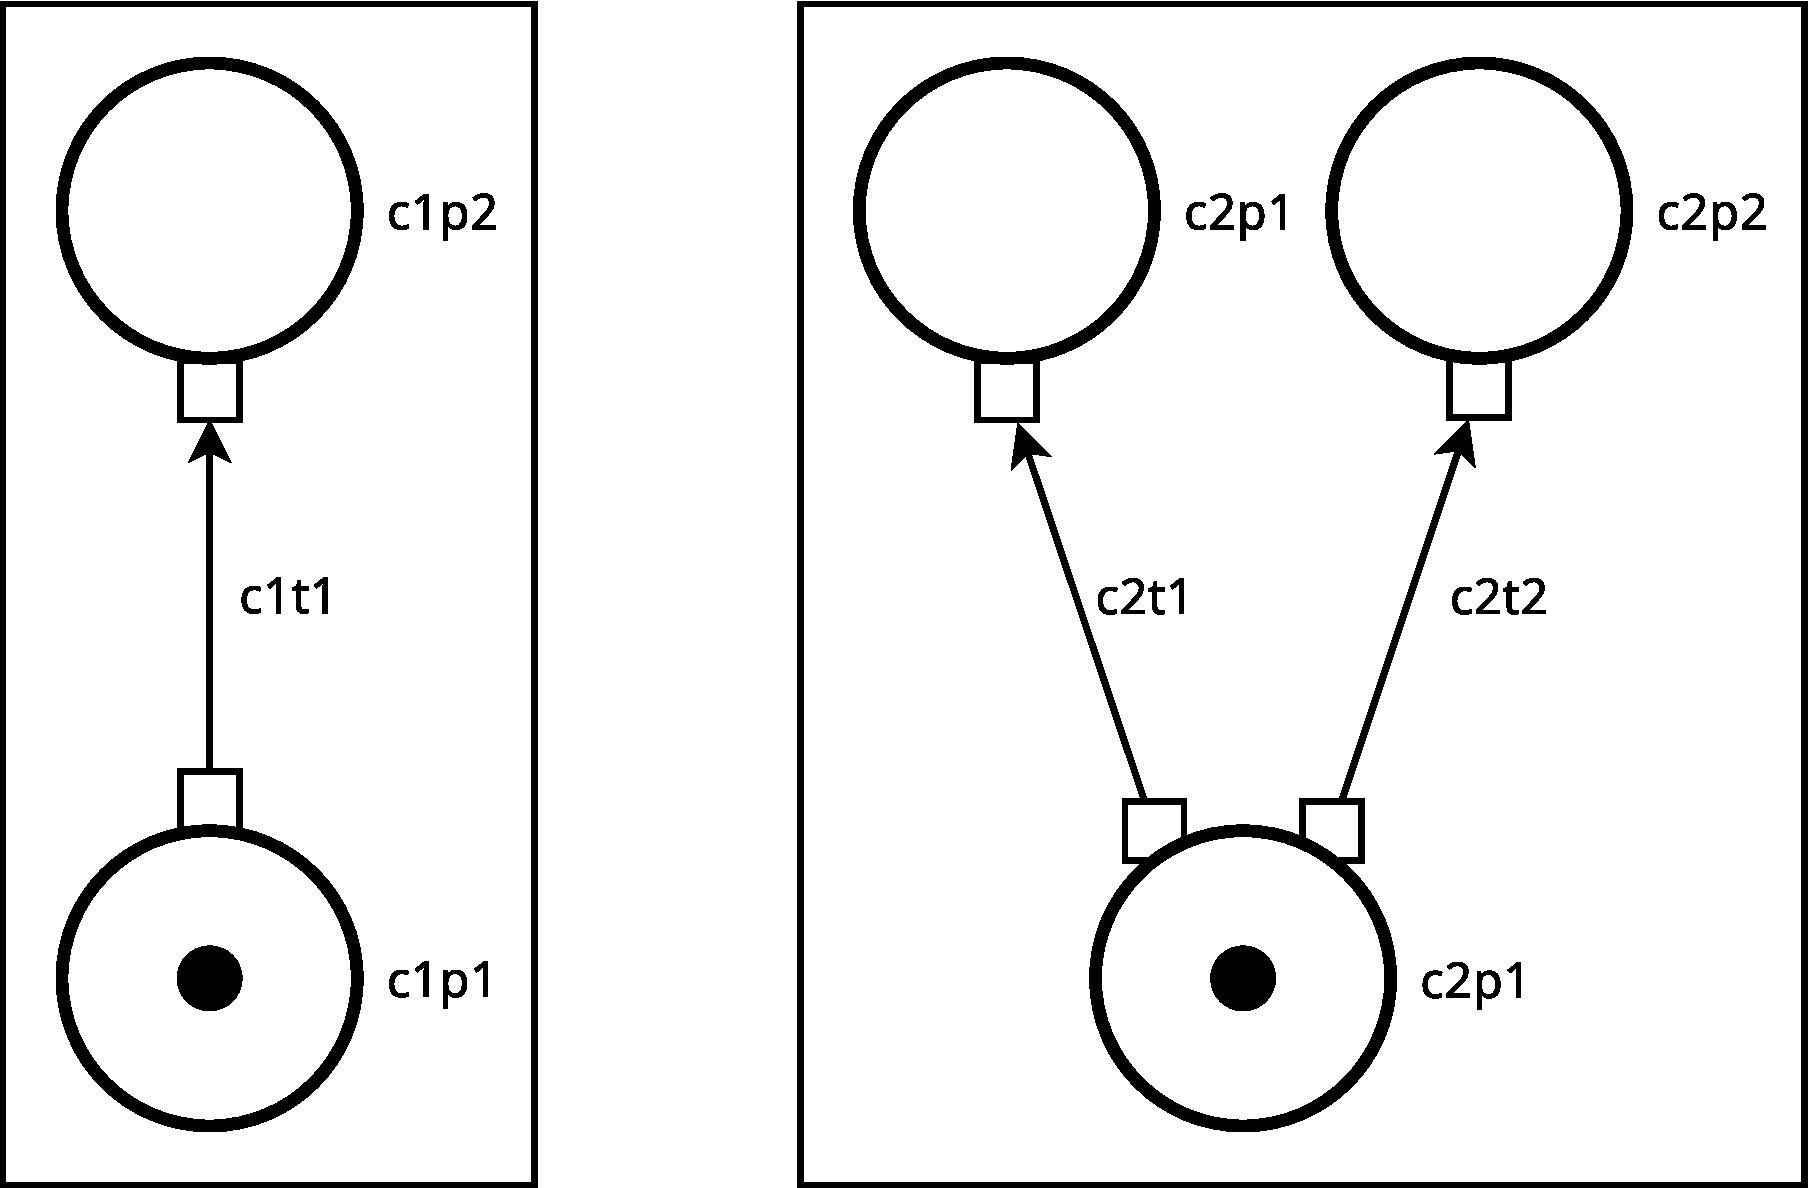
\includegraphics[scale=0.15]{images/perf_source_sink.pdf}
    \end{minipage}
  }
  \\
  
  \subfloat[Dependency graph]{%
    \fcolorbox{black!20}{white}{
      \begin{minipage}[c]{0.95\columnwidth}%
        \centering
        \begin{tikzpicture}[node distance=1.7cm]
          \node (c1p2l) [] {$v_\text{c1p2}^\text{leav}$};
          \node (c1p2) [below =15pt of c1p2l,yshift=-0.3cm] {$v_\text{p1p2}^\text{place}$};
          \node (c1t1e) [below =15pt of c1p2] {$v_\text{c1t1}^\text{end}$};
          \node (c1t1) [below =15pt of c1t1e] {$v_\text{c1t1}^\text{beg}$};
          \node (c1p1l) [below =15pt of c1t1] {$v_\text{c1p1}^\text{leav}$};
          \node (c1p1) [below =15pt of c1p1l] {$v_\text{c1p1}^\text{place}$};
          \node (c2p2) [right =35pt of c1p2] {$v_\text{c2p2}^\text{place}$};
          \node (c2p2l) [above =15pt of c2p2] {$v_\text{c2p2}^\text{leav}$};
          \node (c2t1e) [below =15pt of c2p2] {$v_\text{c2t1}^\text{end}$};
          \node (c2t1) [below =15pt of c2t1e] {$v_\text{c2t1}^\text{beg}$};
          \node (c2p1l) [below =15pt of c2t1, xshift=1.5cm] {$v_\text{c2p1}^\text{leav}$};
          \node (c2p1) [below =15pt of c2p1l] {$v_\text{c2p1}^\text{place}$};
          
          \node (c2p3) [right =35pt of c2p2] {$v_\text{c2p3}^\text{place}$};
          \node (c2p3l) [above =15pt of c2p3, yshift=0.3cm] {$v_\text{c2p3}^\text{leav}$};
          \node (c2t2e) [below =15pt of c2p3] {$v_\text{c2t2}^\text{end}$};
          \node (c2t2) [below =15pt of c2t2e] {$v_\text{c2t2}^\text{beg}$};
          
          \node (source) [below =15pt of c2p1, xshift=-1.8cm] {$v^\text{source}$};
          \node (sink) [above =20pt of c2p2l] {$v^\text{sink}$};
          
          \draw [->] (c1p1) -- (c1p1l) node[midway, right, scale=0.7] {$0$};
          \draw [->] (c1p2) -- (c1p2l) node[midway, right, scale=0.7] {$0$};
          \draw [->] (c2p1) -- (c2p1l) node[midway, right, scale=0.7] {$0$};
          \draw [->] (c2p2) -- (c2p2l) node[midway, right, scale=0.7] {$0$};
          \draw [->] (c2p3) -- (c2p3l) node[midway, right, scale=0.7] {$0$};
          \draw [->] (c1t1) -- (c1t1e) node[midway, right, scale=0.7] {$time(\text{c1t1})$};
          \draw [->] (c2t1) -- (c2t1e) node[midway, right, scale=0.7] {$time(\text{c2t1})$};
          \draw [->] (c2t2) -- (c2t2e) node[midway, right, scale=0.7] {$time(\text{c2t2})$};
          \draw [->] (c1p1l) -- (c1t1) node[midway, right, scale=0.7] {$0$};
          \draw [->] (c2p1l) -- (c2t1) node[midway, right, scale=0.7] {$0$};
          \draw [->] (c2p1l) -- (c2t2) node[midway, right, scale=0.7] {$0$};
          \draw [->] (c1t1e) -- (c1p2) node[midway, right, scale=0.7] {$0$};
          \draw [->] (c2t1e) -- (c2p2) node[midway, right, scale=0.7] {$0$};
          \draw [->] (c2t2e) -- (c2p3) node[midway, right, scale=0.7] {$0$};
          \draw [->] (source.west) to[bend left] node[midway, above, scale=0.7]{$0$} (c1p1.south);
          \draw [->] (source.east) to[bend right] node[midway, above, scale=0.7] {$0$}(c2p1.south);
          \draw [->] (c1p2) -- (sink) node[midway, right, scale=0.7] {$0$};
          \draw [->] (c2p2) to[bend right] node[midway, right, scale=0.7] {$0$}(sink);
          \draw [->] (c2p3) -- (sink) node[midway, right, scale=0.7] {$0$};
        \end{tikzpicture}
      \end{minipage}
    }
  }
  \caption{Transofrmation example fro mtwo components without ports to
    its equivalent execution flow graph}
  \label{fig:source_sink_graph}
\end{figure}

Finally, we define $Ass$ as the union of all of these. 
\[
A=A_\Pi\cup A_{\Theta}\cup A_{D}\cup A_{S}\cup A_{I}\cup A_{F}
\]

%--------------------------------------
\subsection{Time estimation}
%--------------------------------------

In the following, we denote $DG_{Ass}=(V,A)$ the dependency graph corresponding
to assembly $A=(C,L_S,L_D)$, and $DG_c$ the part of a dependency graph
corresponding to component $c \in C$.

We define the time estimation of the execution of the \mad assembly $Ass$
to be the length of a longest path between $v^\text{source}$ and
$v^\text{sink}$ in $DG(ass)$.

\begin{lemma}
 In $DG(ass)$, if $v^\text{sink}$ is reachable from $v^\text{source}$ and there
 are no cycles, then the time estimation for $Ass$ is well-defined.
 \label{lemma:well_defined}
\end{lemma}

\begin{proof}
 If $v^\text{sink}$ is reachable from $v^\text{source}$, there exists at least
 one path from $v^\text{source}$ to  $v^\text{sink}$. Because there are no
 cycles, the number of paths between $v^\text{source}$ and $v^\text{sink}$ is
 finite. Because all the paths have a weight, the set of longest paths is
 well-defined (and not empty). Therefore the length of a longest path is
 well-defined.
\end{proof}

\begin{lemma}
 In a component $c \in C$, if place $\pi_t \in \Pi$ is reachable from place
 $\pi_s \in \Pi$ (distinct from $\pi_t$), then $v_{\pi_t}^{place}$
 is reachable from $v_{\pi_s}^{place}$ in a $DG_c$.
 \label{lemma:reachable}
\end{lemma}

\begin{proof}
 Consider a path $P$ in the \net of $c \in C$ going from $\pi_s$ to
 $\pi_t$ (this path exists because $\pi_t$ is reachable from
 $\pi_s$). This path is made of a sequence of places connected by
 transitions: $P=(\pi_s,t1,p2,t2,\dots,t_n,\pi_t)$.\\
 By construction, there exists a path\\
 $(v_{\pi_s}^{place},v_{\pi_s}^{leav},v_{t1}^{beg},v_{t1}^{end},v_{p2}^{place},\dots,v_{\pi_t}^{place})
 \in DG_c$.
\end{proof}


\begin{lemma}
 If an assembly $Ass$ has one or more components then $v^\text{sink}$ is
 reachable from $v^\text{source}$ in $DG_{Ass}$.
 \label{lemma:source_sink}
\end{lemma}

\begin{proof}
 Let us consider one component $c \in C$, its initial place $\pi_i$ and one of
 its final places $\pi_f$. By construction, $v_{\pi_i}^\text{place}$ is
 reachable from $v^\text{source}$, and $v^\text{sink}$ is reachable from
 $v_{\pi_f}^\text{place}$ in the dependency graph of an assembly containing this
 component. The last thing to prove is that $v_{\pi_f}^\text{place}$ is reachable
 from $v_{\pi_i}^\text{place}$ in $DG_c$.
 The end of the execution of a \mad component is defined as
 when all its tokens are in final places, \ie when there are no more
 transitions to perform. Therefore, by definition $\pi_f$ is
 necessarily reachable from $\pi_i$ in the \net of $c \in C$.
 We conclude by applying Lemma~\ref{lemma:reachable}.
\end{proof}

\begin{lemma}
 If a component $c \in C$ is well-formed then $DG_c$ has no cycle.
 \label{lemma:no_cycles_component}
\end{lemma}

\begin{proof}
 By construction, in $DG_c$ the vertices and arcs corresponding to places do
 not form cycles and are disjoint, so they cannot produce a cycle by themselves.
 Likewise, the arcs corresponding to port bindings have either their source
 vertex or their destination vertex of degree 1, so they cannot produce a cycle.
 Only the arcs corresponding to transitions can produce cycles. Moreover, the
 arcs in $DG_c$ connect only the vertices corresponding to the places which
 are connected in the \net. This means that if there is a cycle in $DG_c$,
 there is a cycle in the \net. However, the \net of a well-formed \mad component
 has no cycle. Therefore there are no cycles in $DG_c$.
\end{proof}

\begin{lemma}
 In an assembly $Ass$ of well-formed components with no deadlocks, if each port
 is bound to at most one element (place, transition or group) and if
 $\left|g_{in}(g)\right|\leq 1$ and $\left|g_{out}(g)\right|\leq 1$ for each group
 $g$ in $Ass$ then the $DG_{Ass}$ has no cycles.
 \label{lemma:no_cycles_assembly}
\end{lemma}

\begin{proof}
 By Lemma~\ref{lemma:no_cycles_component}, we have that the dependency graph
 of all the components in $Ass$ have no cycles.
 Then, the only way a cycle may exist in $DG_{Ass}$ is if the vertices and arcs
 corresponding to connections cause a cycle to exist.
 This may be acheived in two ways: because of a single service port bound to
 group $g$ if $\left|g_{out}(g)\right|>0$ (which implies by hypothesis
 $\left|g_{out}(g)\right|=1$); or because of two or more use and provide ports.
 First, because $\left|g_{out}(g)\right|=1$ (we consider $\pi_{out}$ to be the only
 place in $g_{out}(g)$), and because by construction $v_{\pi_{out}}^{leav}$ is
 reachable from $v_{\pi_{in}}^{place}$ (where $\pi_{in}$ is the only place in $g_{in}(g)$,
 then $v_{\pi_{in}}^{place}$ is not reachable from $v_{\pi_{out}}^{leav}$ (otherwise
 there would be a cycle in the dependency graph of the component). Second, a
 cycle can be caused by multiple connections if there are \emph{crossing
 dependencies} (see Figure~\ref{fig:deadlock}). However, this would create a
 deadlock in the assembly, which is not possible by hypothesis.
\end{proof}

\begin{figure}[t]
  \begin{center}
    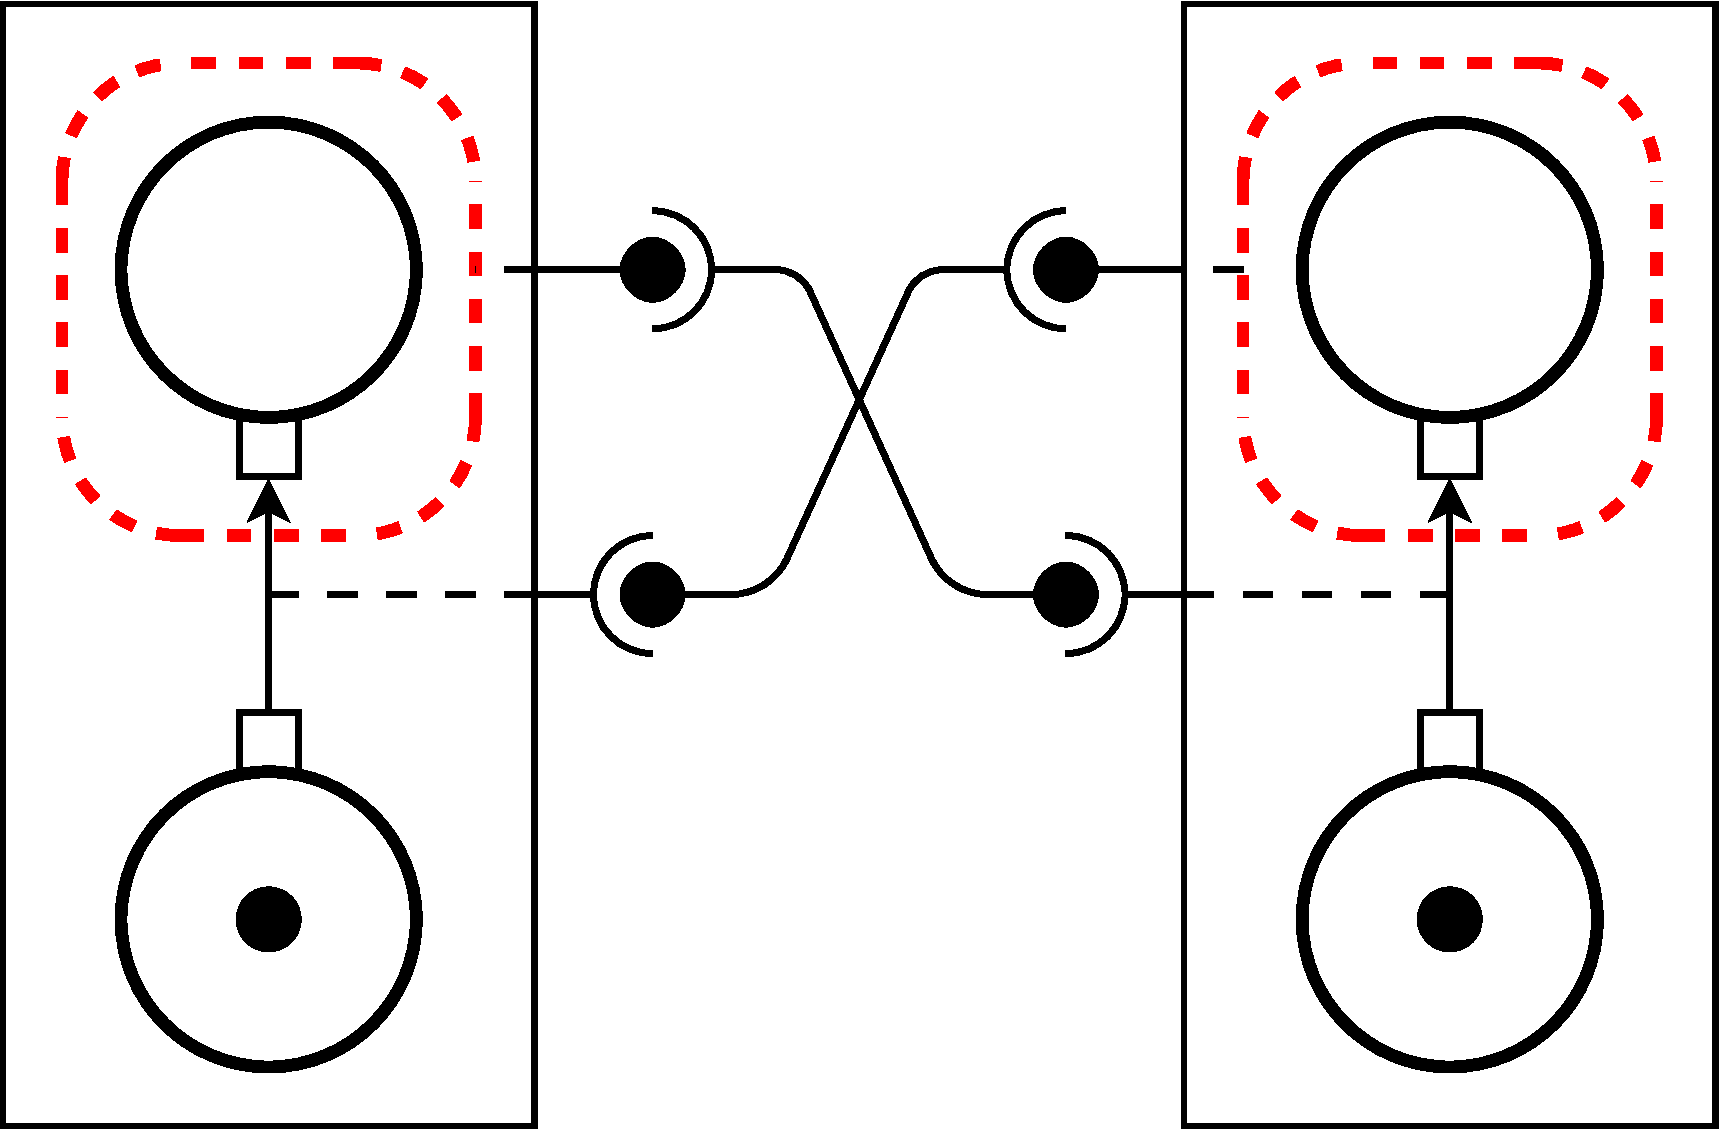
\includegraphics[width=0.5\linewidth]{./images/deadlock.pdf}
  \end{center}
  \caption{Example of an invalid assembly: crossing dependencies cause a deadlock.}
  \label{fig:deadlock}
\end{figure}

\begin{theorem}
 In an assembly $Ass$ of one or more well-formed components with no deadlocks,
 if each port is bound to at most one element (place, transition or group) and if
 $\left|g_{in}(g)\right|\leq 1$ and $\left|g_{out}(g)\right|\leq 1$ for each group
 $g$ in $Ass$, then the time estimation obtained using $DG_{Ass}$ is well-defined.
 \label{theorem:well_defined}
\end{theorem}

\begin{proof}
 By applying Lemma~\ref{lemma:source_sink}, we know that $v^\text{sink}$ is reachable
 from $v^\text{source}$. By applying Lemma~\ref{lemma:no_cycles_assembly}, we know
 that there are no cycles in $DG_{Ass}$. We conclude by applying
 Lemma~\ref{lemma:well_defined}.
\end{proof}

\paragraph{Remark}

The restrictions imposed in \ref{theorem:well_defined} are here to consider only
assemblies for which the structure of the dependency graph does not change
depending on the duration of the transitions. To handle arbitrary assemblies,
a more complex performance model is needed, which is left as future work. In
practice, we expect most real-life assemblies to fulfill these requirements.
In particular, all of the assemblies presented in this article do.


\subsection{Complexity}

We now determine the size complexity of $DG_{Ass}=(V,A)$ and the time
complexity of computing the time estimation.

First, we notice that
$|V| \in \mathcal{O}\left(\left|\pi^*\right|+\left|\theta^*\right|+\left|S_{p^*}\right|+\left|D_{p^*}\right|\right)$
and
$|A| \in \mathcal{O}\left(\left|\pi^*\right|+\left|\theta^*\right|+\left|B_{S_p}\right|+\left|B_{D_p}\right|+\left|B_{S_u}\right|\times\left|L_S\right|\right.$ \\
$\left.+\left|B_{D_u}\right|\times\left|L_D\right|\right)$
.

Because $DG_{Ass}$ is a a directed acyclic graph, finding the longest path
between $v^\text{source}$ and $v^\text{sink}$, \ie finding a time estimation,
can be done in $\mathcal{O}(|V|+|A|)$ by sorting the
vertices topologically and iterating through them, computing their maximum
distance from the source using the one of their parents.

